\section{Discussion and outlook}%
\label{sec:result_discussion}

\todo[inline]{Update results:\\
  CMS overview: \url{https://arxiv.org/pdf/2207.00043.pdf}\\
  ATLAS overview:   \url{https://cds.cern.ch/record/2815513/files/HDBS-2022-03-002.pdf}
}

\todo[inline]{Prospects?\\
  \url{https://cds.cern.ch/record/2798448/files/ATL-PHYS-PUB-2021-044.pdf}\\
  \url{https://cds.cern.ch/record/2802127/files/ATL-PHYS-PUB-2022-005.pdf}
}

\todo[inline]{Make this a separate chapter and include \klambda discussions?}

The results obtained as part of the searches for non-resonant SM \HH
production and resonant production via narrow width scalar bosons are
discussed in the following.

Both searches are largely limited by data statistical uncertainties
which represent the majority of the uncertainty on extracted signal
strengths or cross sections. Systematic uncertainties are
comparatively small for the search for non-resonant SM \HH production
and resonant production at intermediate to high masses. Only for the
search for low mass scalar resonances uncertainties from systematic
sources are comparable to data statistical uncertainties, however,
they do not solely limit the final result.

The largest improvements are expected from increases in the integrated
luminosity expected for Run~3 of the LHC and beyond. The prospects of
searches for Higgs boson pairs for Run~4 (high luminosity LHC) studied
by the ATLAS collaboration
in~\cite{ATL-PHYS-PUB-2021-044,ATL-PHYS-PUB-2022-005} are briefly
discussed providing an outlook for future searches.

% Or by further relaxing the selection requirements yielding larger
% signal acceptance. Although this would also increase the background
% and thus might not correspond to a net improvement of the results.

\subsection{Search for non-resonant production of Higgs boson pairs in
  the SM}

The search presented in this work provides the most stringent expected
upper limits on the signal strength of SM \HH production via \ggF and
VBF for analysis targeting a single final state. This result is put
into context by summarising past and present results of direct SM \HH
searches by the ATLAS collaboration
in~\Cref{fig:atlas_run2_hh_results} and with the results of the CMS
collaboration in~\Cref{tab:cms_nonresonant} for analyses of the Run~2
dataset of $pp$-collisions.

\begin{figure}[tbp]
  \centering

  \begin{subfigure}[b]{0.53\textwidth}
    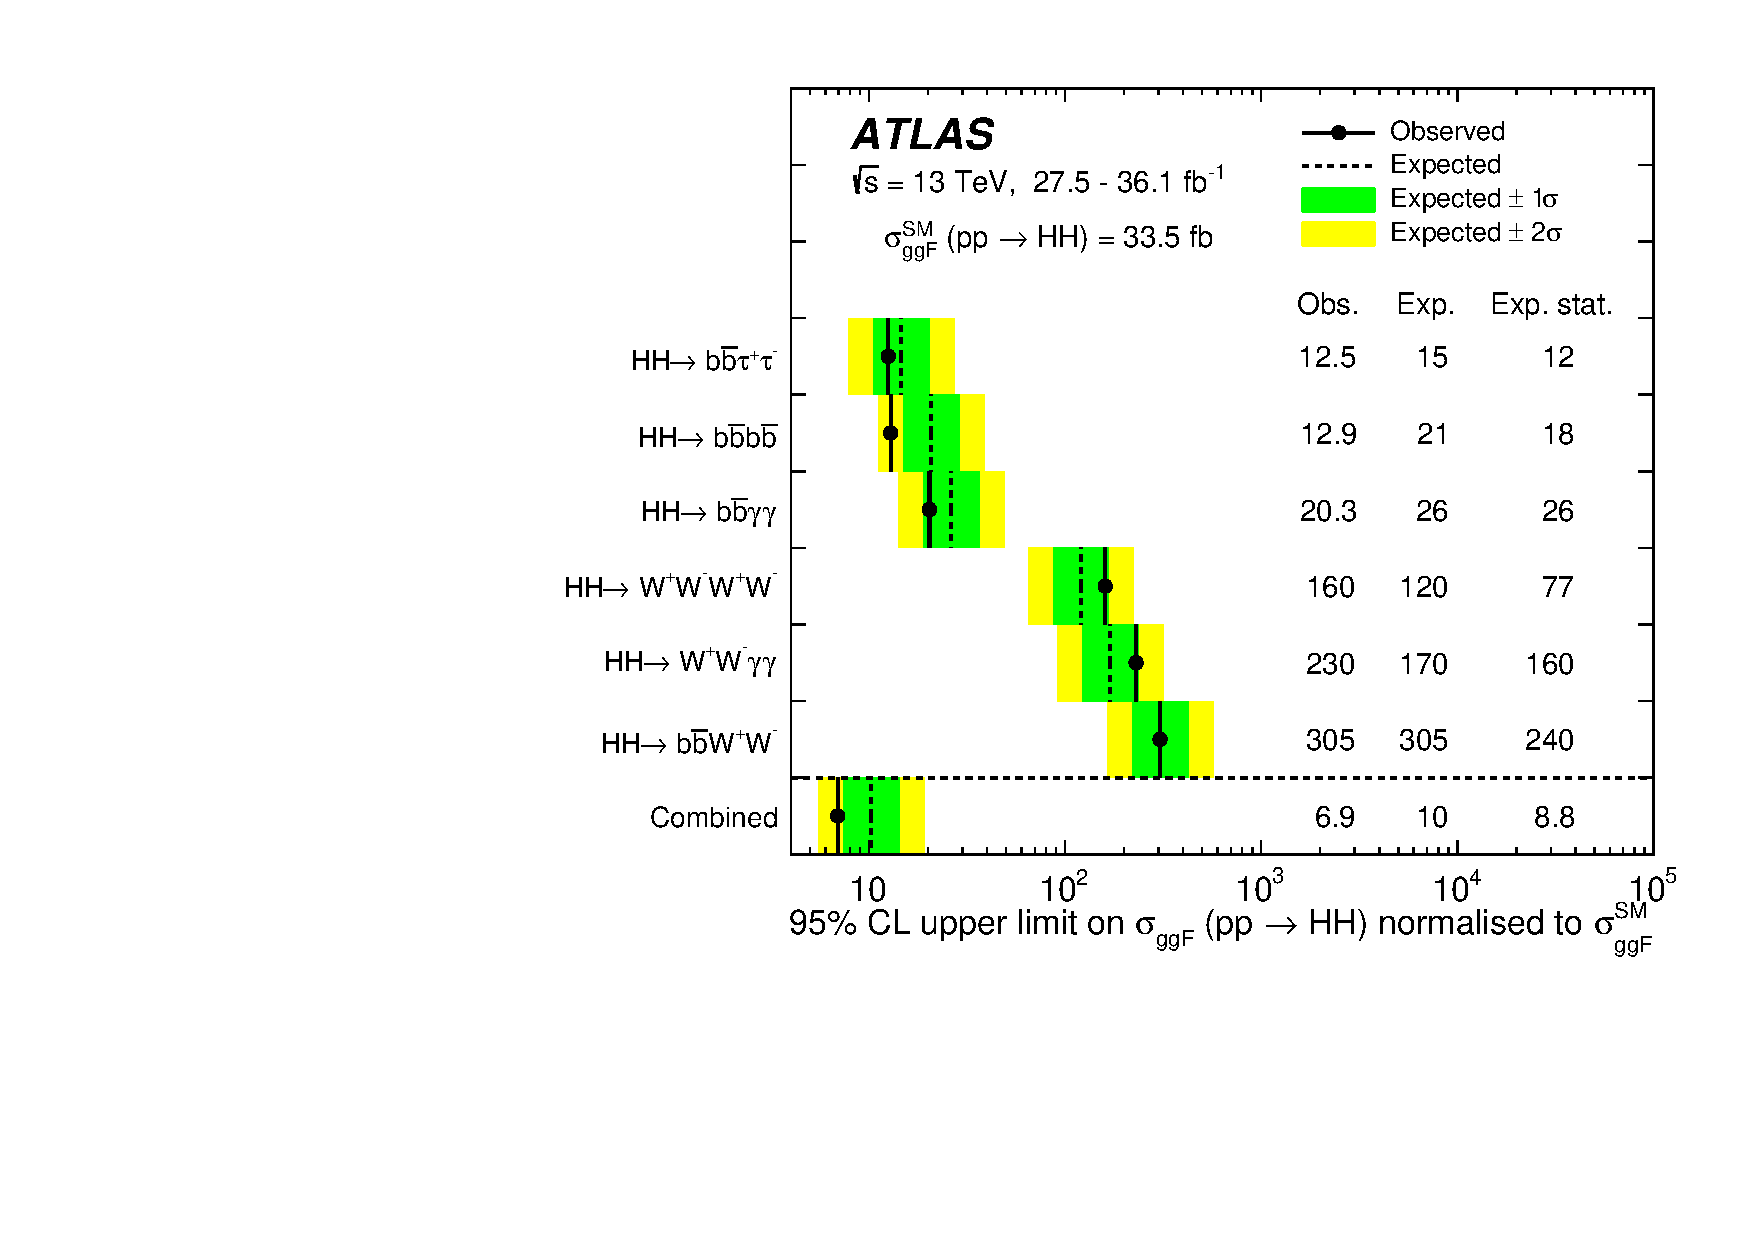
\includegraphics[width=\textwidth]{discussion/results_36ifb}

    \subcaption{Partial Run~2 dataset with an integrated luminosity of \num{27.5} -
      \SI{36.1}{\per\femto\barn}~\cite{HDBS-2018-58}}%
    \label{fig:atlas_run2_36ifb}
  \end{subfigure}\hfill%
  \begin{subfigure}[b]{0.46\textwidth}
    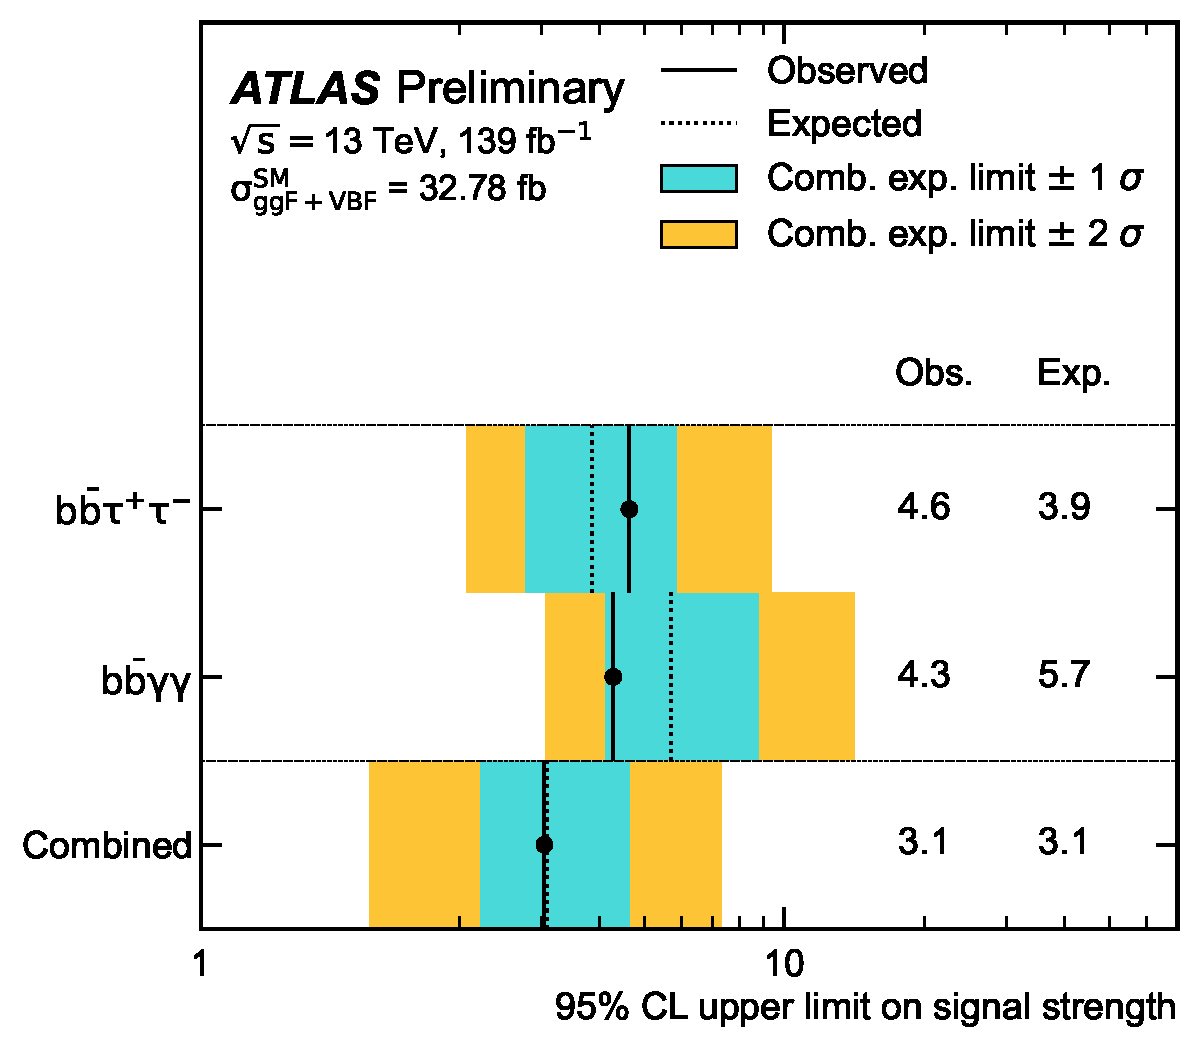
\includegraphics[width=\textwidth]{discussion/results_139ifb}

    \subcaption[margin=5em]{Full Run~2 dataset with an integrated luminosity
      of~\SI{139}{\per\femto\barn}~\cite{ATLAS-CONF-2021-052}}%
    \label{fig:atlas_run2_139ifb}
  \end{subfigure}

  \caption{Comparison of ATLAS results for searches for non-resonant
    SM \HH production from the beginning (a) and end of Run~2 (b) of
    the LHC. Upper limits are shown in terms of the signal strength of
    SM \HH production via \ggF neglecting the VBF production mode in
    (a) and in terms of the combined signal strength of \ggF and VBF
    production mode in (b). Both results are still comparable due to
    the small cross section of VBF \HH production. Additionally, the
    assumed SM \HH cross sections changed between results due to the
    availability of improved theoretical predictions.  Note the
    different results for bbtautau. }
  \label{fig:atlas_run2_hh_results}
  \todo[inline]{Make my own plot / table for RHS including bbWW and
    possibly 4b? 4b obs.\ 5.4 (exp.\ 8.1)}
\end{figure}

\begin{table}[tbp]
  \centering

  \todo[inline]{Mark preliminary results?}

  \caption{Table of CMS results of searches for non-resonant
    production of Higgs boson pairs with an integrated luminosity of
    \SI{138}{\per\femto\barn}. Upper limits are shown at
    \SI{95}{\percent} CL on the signal strength of the combination of
    the \ggF and VBF production modes.}%
  \label{tab:cms_nonresonant}

  \begin{tabular}{l@{\hskip 2em}SSc}
  \toprule
  \textbf{CMS} (\SI{138}{\per\femto\barn}) & \multicolumn{3}{c}{Upper limit on $\mu_{gg\text{F+VBF}}$ (\SI{95}{\percent} CL)} \\
  \cmidrule{2-4}
  Final state & {Observed} & {Expected} & Reference \\
  \midrule
  $\bbbar\tau^{+}\tau^{-}$ & 3.3 & 5.2 & \cite{CMS-PAS-HIG-20-010} \\
  $\bbbar\gamma\gamma$ & 7.7 & 5.2 & \cite{CMS-HIG-19-018} \\
  $\bbbar\bbbar$ & 3.9 & 7.8 & \cite{CMS-HIG-20-005-PREPRINT} \\
  % Multilepton = ($W^+W^-W^+W^-$, $W^+W^-\tau^+\tau-$, $\tau^+\tau^-\tau^+\tau^-$)
  Multi-lepton  & 21.8 & 19.6 & \cite{CMS-PAS-HIG-21-002} \\
  \bottomrule
\end{tabular}


%%% Local Variables:
%%% mode: latex
%%% TeX-master: "../phd_thesis"
%%% End:

\end{table}

With the currently available dataset and experimental constraints (due
to triggers, reconstruction, identification / isolation) of the ATLAS
experiment for Run~2 of the LHC, the \bbtautau channel achieves a
trade-off between the competing \bbyy and \bbbb channels regarding the
search for SM \HH production. While the \bbyy channel provides access
to events with low \mHH due to the ability to trigger on the signature
of photons with low momentum thresholds (this is particularly
advantageous when considering anomalous values of the Higgs boson
self-couplings, cf.~REFERENCE) and a large background rejection due to
the excellent $\gamma\gamma$ mass resolution, it is subject to the
very small $\PHiggs \to \gamma\gamma$ branching ratio. In contrast,
the largest fraction of SM \HH events are expected in the \bbbb final
state, however, the measurement of SM \HH production in this channel
is challenging due to the fully hadronic final state being subject to
large multi-jet backgrounds and difficulties in selecting signal
candidate events at trigger-level\footnote{There are also
  combinatorial difficulties in reconstructing $\PHiggs \to \bbbar$
  candidates in the \bbbb channel where it can be ambiguous
  (particularly at low \mHH) how $b$-jets are paired into Higgs boson
  candidates. However, SM \HH production is produced at sufficiently
  high \mHH such that this is not really a huge issue.}. The \bbtautau
final state, particularly in the \hadhad channel due to less prevalence
of \ttbar backgrounds compared to the \lephad channel, is very
sensitive to SM \HH production as signal events can be efficiently
selected using \tauhadvis triggers due to their hard \mHH
spectrum. The presence of \tauhadvis (and electrons / muons) provides
large rejection power against multi-jet backgrounds compared to the
\bbbb channel. Moreover, the fraction of SM \HH events decaying into
\bbtautau final states is significantly larger than that of \bbyy.

In~\Cref{fig:atlas_run2_36ifb,fig:atlas_run2_139ifb} a comparison
between searches for SM \HH production using the partial and full
Run~2 $pp$-collision dataset collected with the ATLAS detector is
given. The search for SM \HH production in the \bbtautau final state
using data collected at the beginning of Run~2 of the LHC
(\SI{36.1}{\per\femto\barn}) yielded an expected upper limit on
$\mu_{\ggF}$ of 14.8~\cite{HIGG-2016-16-witherratum}. While upper
limits are set on a different parameter and different theory cross
sections for the signal are assumed, the results can still be compared
to the one obtained using the full Run~2 $pp$-collision dataset
(\SI{139}{\per\femto\barn}) since the change cross section is small
and the contribution of the VBF production mode can be neglected for
the purpose of this comparison. The analysis of the full Run~2
$pp$-collision dataset presented in this work yields an expected upper
limit on $\mu_{\ggF+\text{VBF}}$ of 3.9, far exceeding the expectation
from a naive scaling of the previous result according to the increase
in integrated luminosity which would yield an expected upper limit of
about~7.\footnote{Assuming a purely statistically limited measurement
  that scales with integrated luminosity like a Poisson counting
  experiment. The change in the upper limit depends on the expected
  number of background events and thus cannot be solely described by
  the change in integrated luminosity. Depending on the scenario, the
  extrapolation of the upper limit of \num{14.8} from
  \SI{36.1}{\per\femto\barn} to \SI{139}{\per\femto\barn} ranges
  between \num{6.5} and \num{7.5}.}  This improvement is primarily due
to two reasons:
\begin{itemize}

\item Large improvements in signal sensitivity due to improvements in
  $b$-jet tagging, \tauhadvis reconstruction and identification, which
  allowed to relax identification requirements while maintaining
  background rates comparable to the previous analysis. %
  %                      Old        New
  % LepHad (SLT+LTT)     3.2 %      5.1 %
  % HadHad               1.9 %      4.1 %
  As a result, the signal acceptance improved by a factor of about 2
  (about 1.5) in the \hadhad (\lephad) channel.

\item The increase in integrated luminosity of the collected dataset
  increases the population of signal-like phase spaces allowing for
  better exploitation of the distinct signature of Higgs boson pair
  production.

  This is a side effect of the constraints imposed on the re-binning
  algorithms applied to the MVA discriminants. The limits on the
  minimum number of background events (expected) and maximum
  statistical uncertainty on the background estimate for a good bin
  introduce a dependency of the re-binning algorithm on the integrated
  luminosity of data and simulation. Thus, an increase in integrated
  luminosity allows for narrower bins in the high MVA score region
  improving signal sensitivity. This is not a general feature but due
  to the large discrimination power of the MVA discriminants used to
  extract the SM \HH signal.\todo{It would be good to know how large
    this effect is?}
\end{itemize}

\todo[inline]{Comparison with CMS results. Why is ATLAS better?}

An outlook on the future of non-resonant SM \HH searches with the
ATLAS experiment is provided by an extrapolation of the search
presented in this thesis to the end of the HL-LHC project. The HL-LHC
is expected to deliver an integrated luminosity of
\SI{3000}{\per\femto\barn} (optimistic scenarios up to
\SI{4000}{\per\femto\barn}) of $pp$-collision data at
$\sqrt{s} = \SI{14}{\TeV}$~\cite{hllhc:tdr}. The ATLAS collaboration
performed an extrapolation of the non-resonant SM \HH search in the
\bbtautau channel as part of Ref.~\cite{ATL-PHYS-PUB-2021-044} to the
conditions at the end of HL-LHC data-taking. This extrapolation is
conducted under the assumption that the performance of the ATLAS
detector can be maintained at the level of the Run~2 performance in
spite of the large increase in instantaneous luminosity at the
HL-LHC. The analysis is extrapolated to an integrated luminosity of
\SI{3000}{\per\femto\barn}, accounting for changes in cross sections
for signal and background processes due to the increase in $\sqrt{s}$
from \SI{13}{\TeV} to \SI{14}{\TeV}. The evolution of systematic
uncertainties follows the ``baseline'' scenario outlined in
Refs.~\cite{ATL-PHYS-PUB-2019-005,ATL-PHYS-PUB-2019-006}. Under these
assumptions the search for non-resonant SM \HH production in the
\bbtautau channel is extrapolated to yield a discovery significance of
$2.8\,\sigma$ (assuming the SM) at the end of the
HL-LHC~\cite{ATL-PHYS-PUB-2021-044}. Thus evidence for non-resonant SM
\HH production for a search in solely in the \bbtautau channel is in
reach provided some improvements can be made.

Extrapolations under similar assumptions were performed for the \bbyy
search channel yielding a significance of
$2.2\,\sigma$~\cite{ATL-PHYS-PUB-2022-001}. Further, the prospects of
combining the \bbtautau and \bbyy searches at the end of the HL-LHC
were investigated in Ref.~\cite{ATL-PHYS-PUB-2022-005} suggesting that
evidence for SM \HH production can be obtained with a discovery
significance of $3.2\,\sigma$ for the combination of both channels. A
discovery ($5\,\sigma$) of SM \HH production at the end of the HL-LHC
is realistic but will likely require the combination of the most
sensitive channels across both the ATLAS and CMS
collaborations.\footnote{For prospects of SM \HH searches by the CMS
  collaboration see Refs.~\cite{CMS-PAS-FTR-18-019} and
  \cite{CMS-PAS-FTR-21-004} from the beginning and the end of Run~2,
  respectively.}  However, the HL-LHC prospect studies by both
collaborations suggest that some sensitivity improvements will be
necessary to claim discovery of SM \HH production with the dataset
collected at the HL-LHC provided the assumptions of the extrapolations
hold.
% https://cms-results.web.cern.ch/cms-results/public-results/preliminary-results/FTR/index.html

\todo[inline]{Check
  \url{https://cds.cern.ch/record/2805993/files/ATL-PHYS-PUB-2022-018.pdf}
  for ATLAS+CMS combination discovery significance. And this:
  \url{https://cds.cern.ch/record/2703572/files/94-87-PB.pdf} (4
  sigma).  }

\todo[inline]{\url{https://twiki.cern.ch/twiki/bin/view/CMSPublic/SummaryResultsHIG}}

\subsection{Search for resonant production of Higgs boson pairs}

The sensitivity of the \bbtautau search channel to resonant production
of Higgs boson pairs via narrow scalar resonances is complementary to
the \bbyy and \bbbb channels. \Cref{fig:resonant_hh_comb_limits} shows
a comparison of upper limits on $\sigma(X \to \HH)$ for all three
channels as well as their statistical combination. The \bbtautau
channel provides the largest signal sensitivity for intermediate \mX
ranging from \SIrange{400}{800}{\GeV}. The sensitivity for smaller
(larger) resonance masses is driven by the \bbyy (\bbbb) channel
instead. This behaviour is analogous to the discussion of the previous
section where \bbyy is advantageous in accessing low masses due to the
use of photon triggers and \bbbb at high mass due to the large
$H \to \bbbar$ branching ratio and the large Lorentz boost of the
Higgs bosons resolving the combinatorial ambiguities in constructing
the Higgs boson candidates.

\begin{figure}[htbp]
  \centering

  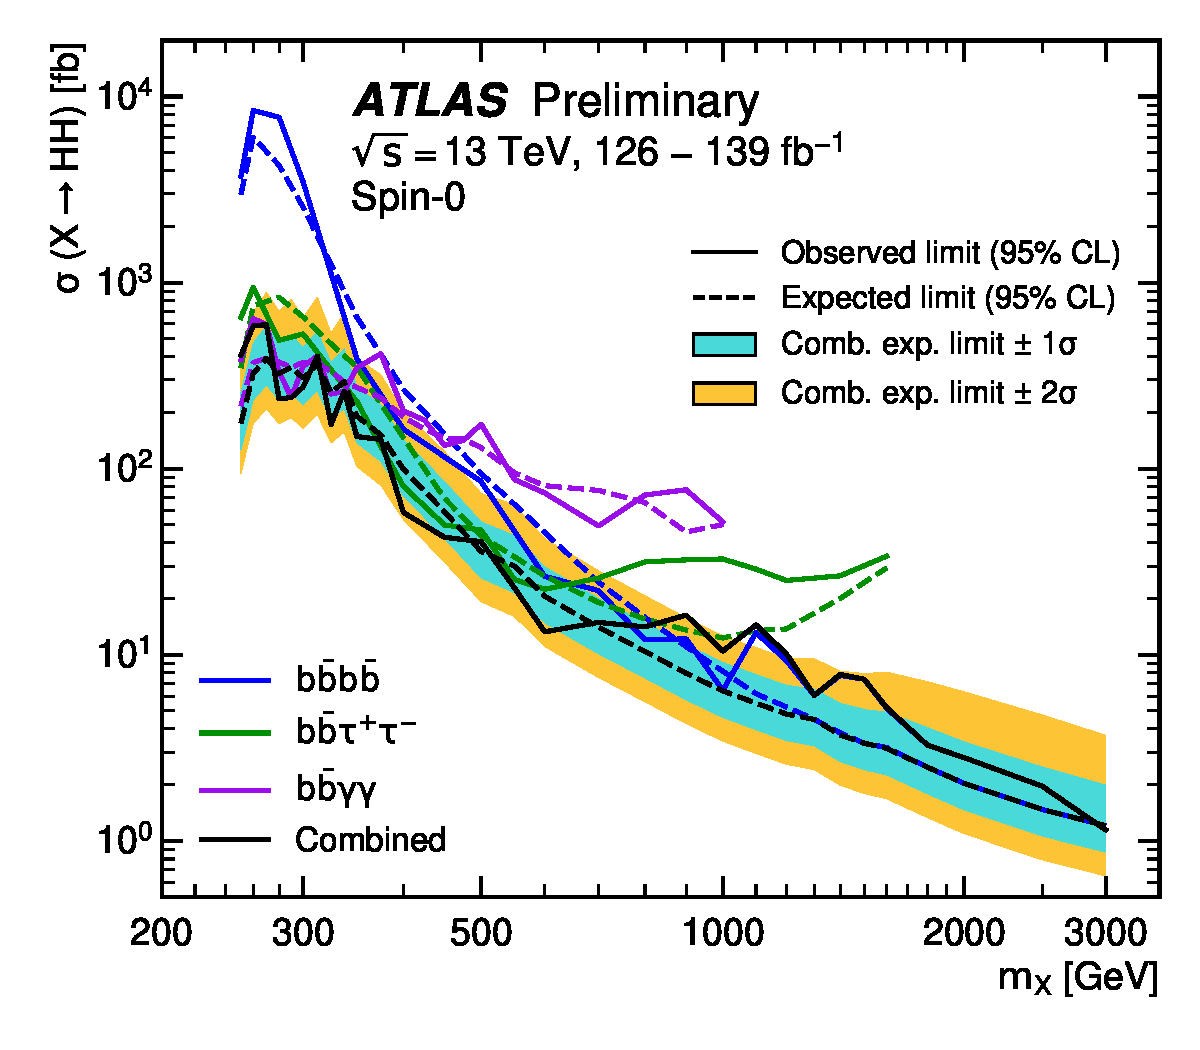
\includegraphics[width=0.55\textwidth]{discussion/limits_resonant_combination}

  \caption{Expected and observed upper limits on $\sigma(X \to \HH)$
    for narrow width scalar resonances $X$ at \SI{95}{\percent}
    \CLs. Upper limits are shown separately for searches in the \bbbb,
    \bbtautau, and \bbyy channels performed with
    \SIrange{126}{139}{\per\femto\barn} of $pp$-collision data taken
    during Run~2 of the LHC. The statistical combination of the three
    measurements is shown in black including its $\pm 1$ and
    $\pm 2\,\sigma$ uncertainty band. The figure is adopted from
    Ref.~\cite{ATLAS-CONF-2021-052}.}
  \label{fig:resonant_hh_comb_limits}
\end{figure}

\todo[inline]{Paragraph about the combination?}

The excess observed for $\mX = \SI{1000}{\GeV}$ in the \bbtautau
channel is compared to the results obtained by the \bbbb analysis to
check the consistency of the results. The best-fit cross section,
expressed in terms of $\sigma(X \to \HH)$, obtained from the \bbtautau
channel measurement is \SIpmerr{17.4}{+7.5}{-6.5}{\femto\barn} for a
signal with a mass of \SI{1000}{\GeV}. This can be compared to the
observed (expected) upper limit of \SI{6.5}{\femto\barn}
(\SI{8.2}{\femto\barn}) at $\mX = \SI{1000}{\GeV}$ set by the search
in the \bbbb channel~\cite{HDBS-2018-41,hepdata.111124}. The cross
section measured in the \bbtautau channel is therefore excluded at
\SI{95}{\percent} CL by the search in the \bbbb final state. This lack
of compatibility is further illustrated in
\Cref{fig:resonant_hh_comb_pvalues} showing the local discovery
significances of the three channels and their combination. While the
incompatibility between the \bbtautau and \bbbb results at
$\mX = \SI{1000}{\GeV}$ reduces the local significance of the
combination, a small excess is observed in the \bbbb channel for
$\mX = \SI{1100}{\GeV}$ which, in combination with the \bbtautau
result, shifts the most significant excess of the combination to
\SI{1100}{\GeV} with a local significance of about
$3.2\,\sigma$~\cite{ATLAS-CONF-2021-052}.

% 4b exclusion (\SIpmerr{8.2}{+1.2}{-0.8}{\femto\barn})

\begin{figure}[htbp]
  \centering

  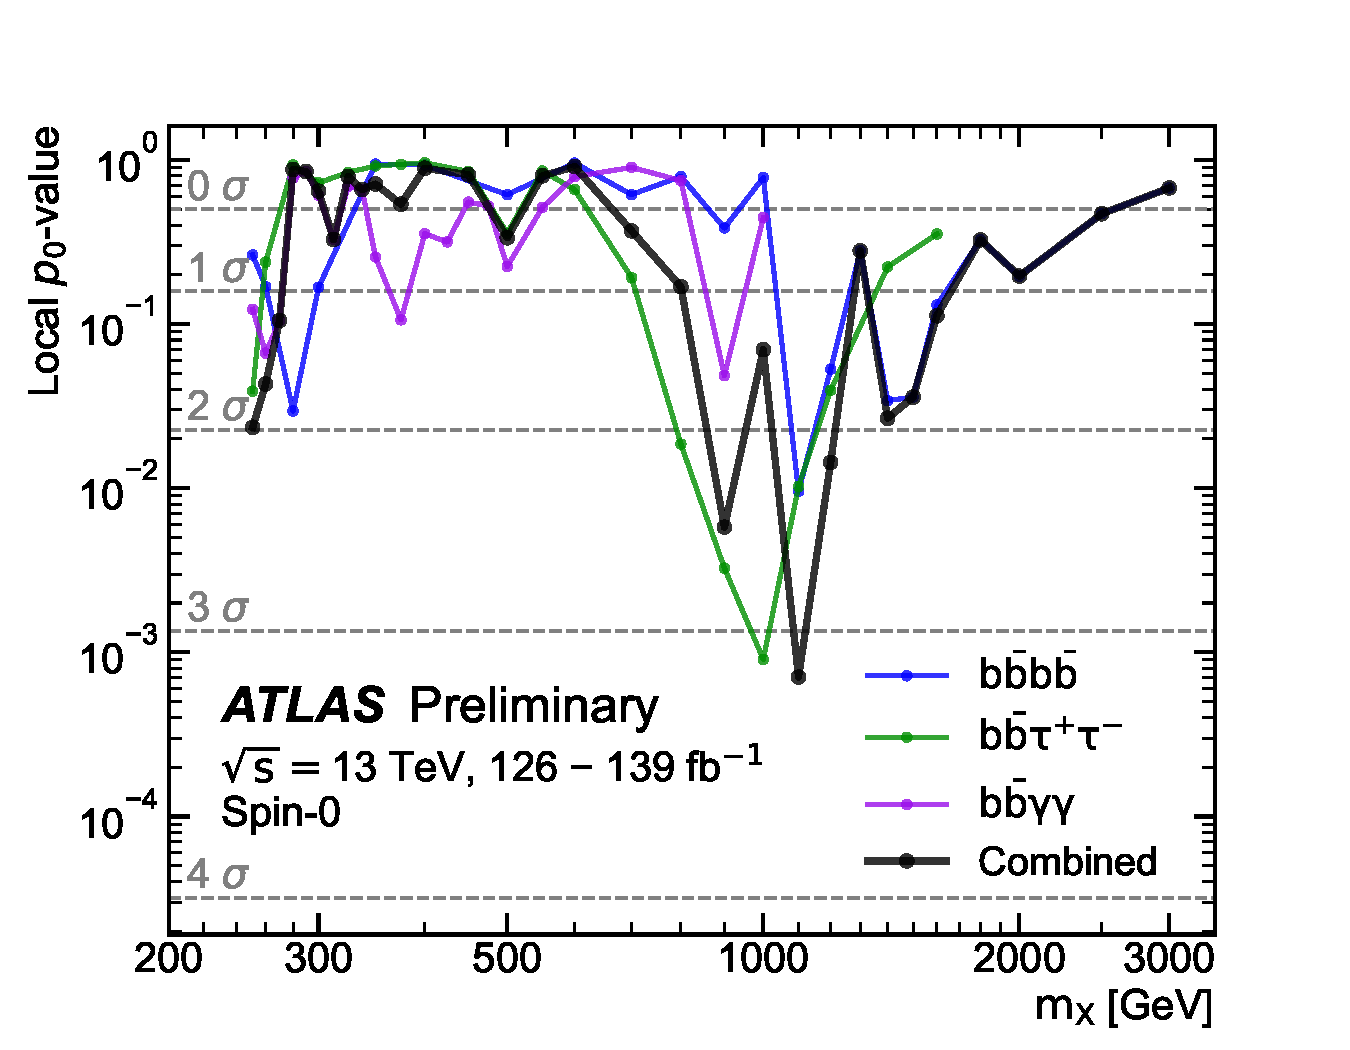
\includegraphics[width=0.55\textwidth]{discussion/pvalues_resonant_combination.pdf}

  \caption{Observed values of the local $p$-values / local
    significances for the \bbbb, \bbtautau, and \bbyy channel and
    their statistical combination for the search for narrow width
    scalar resonances produced via \ggF. The figure is adopted from
    Ref.~\cite{ATLAS-CONF-2021-052}.}
  \label{fig:resonant_hh_comb_pvalues}

  \todo[inline]{The pvalues of the excess do not agree with the
    p-value scan shown earlier.}
\end{figure}

Another comparison is provided by a search for resonant production of
Higgs boson pairs with high momenta targeting final states with
$b$-quarks and one or two light leptons (primarily $\bbbar W^+ W^-$
and $\bbbar \tau^+ \tau^-$) performed by the CMS collaboration in
Ref.~\cite{CMS-B2G-20-007}. This analysis provides very stringent
limits on the production of generic scalar resonances with narrow
width and masses ranging from \SIrange{0.8}{4.5}{\TeV}. Observed
(expected) upper limits on $\sigma(X \to \HH)$ are set at
\SI{4.8}{\femto\barn} and \SI{3.4}{\femto\barn} (\SI{9.6}{\femto\barn}
and \SI{7.1}{\femto\barn}) for resonance masses of \num{1000} and
\SI{1100}{\GeV},
respectively~\cite{CMS-B2G-20-007,hepdata.115024}. This analysis
observes a deficit in data compared to the background prediction for
masses close to \SI{1000}{\GeV}, suggesting that the features observed
by the ATLAS collaboration are coincidental or from other sources.

% CMS resonant results:
%
% HH -> bbWW / bbtautau / bbZZ (boosted bb+l / ll final states)
% https://arxiv.org/pdf/2112.03161.pdf (published JHEP)
%                Obs.             Exp.
% 1000 GeV:      4.8 fb           9.6 fb
% 1100 GeV:      3.4 fb           7.1 fb
%
% - Too good to be true??? Probably fine
%
% HH -> 4b (boosted)
% https://cds.cern.ch/record/2777083/files/B2G-20-004-pas.pdf (preliminary)
%                Obs.             Exp.
% 1000 GeV:      28 fb            15 fb
% 1100 GeV:      9.9 fb           9.4 fb
%
% - Also an excess at 1 TeV (2 sigma ish)
% - None at 1.1 TeV
%
%
% HH -> WWWW, WWtautau, 4tau (multi-lepton)
% https://cds.cern.ch/record/2799151/files/HIG-21-002-pas.pdf (preliminary)
%                Obs.             Exp.
% 1000 GeV:      200-300 fb       100 fb
%
% - 2ish sigma excess but not competitive

In conclusion, the broad excess observed at $\mX = \SI{1000}{\GeV}$ in
the \bbtautau channel with a local (global) significance of
$\num{3.1}\,\sigma$ ($\num{2.0}\,\sigma$) is not statistically
significant after accounting for multiple hypothesis
testing. Additionally, searches for resonant Higgs boson pair
production performed by the CMS collaboration do not corroborate the
excesses observed in this analysis and in the combination of the
\bbbb, \bbtautau, and \bbyy channels.

While the observed excess might have arisen from a statistical
fluctuation of background events, it will be instructive for future
iterations of this search to further scrutinise the background
estimation methodology to rule out that these features are caused by a
systematic mismodelling of the background. A candidate for inspection
would be the \ZHF background, the largest background process in
signal-like bins for high \mX discriminants in both the \hadhad and
\lephad channels, for which the control region measurement of the \ZHF
normalisation could be performed differentially to account for
systematic shifts in the normalisation in certain regions of phase
space. A variable to control for could be the transverse momentum of
the $Z$ boson for which there are indications of systematic effects on
the fitted normalisation (cf.\ REFERENCE APPENDIX). Moreover, a
comparison of reconstruction and identification efficiencies for
highly collinear \tauhadvis between simulation and data would be
further confirm that these topologies are not affected by
miscalibrations of the efficiencies.

% PNN strategy not suitable for cleanly locating the excess.???

%%% Local Variables:
%%% mode: latex
%%% TeX-master: "../../phd_thesis"
%%% End:
